%%%%%%%%%%%%%%%%%%%%%%%%%%%%%%%%%%%%

\section{割合の仮説検定}

%%%%%%%%%%%%%%%%%%%%%%%%%%%%%%%%%%%%

\subsection{仮説検定の枠組み}

%%%%%%%%%%%%%%%%%%%%%%%%%%%%%%%%%%%%

\begin{frame}
\frametitle{思い出してみよう…}

性差別実験：

{\footnotesize
\begin{tabular}{ll  cc c}
  		&				& \multicolumn{2}{c}{\textit{昇進}} \\
\cline{3-4}
							&			& 昇進あり	& 昇進なし	& 合計	\\
\cline{2-5}
\multirow{2}{*}{\textit{性別}}	&男性		& 21	 	& 3		& 24 	\\
							&女性		& 14	 	& 10 	 	& 24 \\
\cline{2-5}
							&合計		& 35		& 13		& 48 \\
\end{tabular}
}

\[ \hat{p}_{\text{男性}} = 21 / 24 \approx 0.88 ~ \text{ および } ~ \hat{p}_{\text{女性}} = 14 / 24 \approx 0.58 \]

考えられる説明：
\begin{itemize}
\item 昇進と性別は\hl{独立}であり、性差別はなく、割合の差は単なる偶然による。$\rightarrow$ \orange{帰無仮説} - {\small （何も起きていない）}
\item 昇進と性別は\hl{従属}であり、性差別があり、割合の差は偶然ではない。$\rightarrow$ \orange{対立仮説} - {\small （何かが起きている）}

\end{itemize}

\end{frame}

%%%%%%%%%%%%%%%%%%%%%%%%%%%%%%%%%%%%

\begin{frame}
\frametitle{結果}

\begin{center}
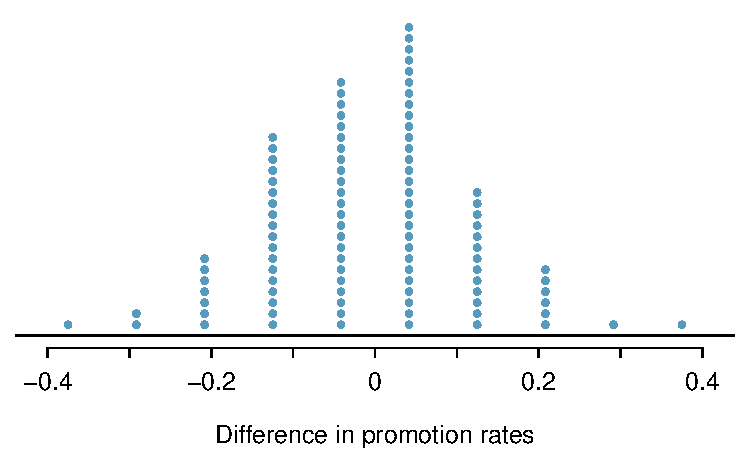
\includegraphics[width=0.75\textwidth]{5-3_ht_prop/figures/discRandDotPlot/discRandDotPlot}
\end{center}

シミュレーションにおいて実際のデータと同等またはそれ以上の極端な結果（男性の昇進率が女性より30\%以上高い）が得られる可能性は非常に低かったため、帰無仮説を棄却して対立仮説を採択することにした。

\end{frame}

%%%%%%%%%%%%%%%%%%%%%%%%%%%%%%%%%%%%

\begin{frame}
\frametitle{まとめ：仮説検定の枠組み}

\begin{itemize}
\item 現状を表す\hl{帰無仮説（$H_0$）}から始める。
\item また、研究上の問い（検定したいこと）を表す\hl{対立仮説（$H_A$）}も設定する。
\item 帰無仮説が真であるという前提のもとで、シミュレーションまたは中心極限定理に基づく伝統的な手法によって仮説検定を行う（次に説明する）。
\item 検定結果が、対立仮説を支持する説得力のある証拠がデータに含まれないことを示す場合は、帰無仮説を維持する。そうでない場合は、帰無仮説を棄却して対立仮説を採択する。
\end{itemize}
割合に関する主張を検定する例を使って、仮説検定の枠組みを正式に紹介する。

\end{frame}

%%%%%%%%%%%%%%%%%%%%%%%%%%%%%%%%%%%

\subsection{信頼区間を用いた仮説検定}

%%%%%%%%%%%%%%%%%%%%%%%%%%%%%%%%%%%%

\begin{frame}
\frametitle{信頼区間を用いた仮説検定}

{\small \dq{先ほど、Facebookが自分の興味を正確に分類していると思うアメリカのFacebookユーザーの割合に対する95\%信頼区間を64\%から67\%と計算した。この信頼区間に基づいて、アメリカのFacebookユーザーの過半数がFacebookによる興味の分類は正確だと思っているという仮説をデータは支持するか？}}

\begin{itemize}

\item 対応する仮説は次の通りである：
\begin{itemize}
\item[$H_0$:] $p = 0.50$：アメリカのFacebookユーザーの50\%がFacebookによる興味の分類は正確だと思っている
\item[$H_A$:] $p > 0.50$：アメリカのFacebookユーザーの50\%以上がFacebookによる興味の分類は正確だと思っている
\end{itemize}

\item 帰無値が区間に含まれていない $\rightarrow$ 帰無仮説を棄却する。

\item これは仮説検定の簡便な方法だが、帰無仮説のもとでの特定の結果の可能性（p値）は示さない。

\end{itemize}

\end{frame}

%%%%%%%%%%%%%%%%%%%%%%%%%%%%%%%%%%%%

\subsection{決定誤差}

%%%%%%%%%%%%%%%%%%%%%%%%%%%%%%%%%%%%

\begin{frame}
\frametitle{決定誤差}

\begin{itemize}

\item 仮説検定は完璧ではない。

\item 司法制度では、無実の人が誤って有罪判決を受けたり、有罪の人が無罪放免になったりすることがある。

\item 同様に、統計的仮説検定でも誤った決定をすることがある。

\item 違いは、統計学では誤りを犯す頻度を定量化するための道具があることである。

\end{itemize}

\end{frame}

%%%%%%%%%%%%%%%%%%%%%%%%%%%%%%%%%%%%

\begin{frame}
\frametitle{決定誤差（続き）}

帰無仮説と対立仮説という2つの競合する仮説がある。仮説検定では、どちらが真である可能性が高いかを決定するが、その選択が誤っている場合がある。\\

\begin{center}
\begin{tabular}{l l | c c}
\multicolumn{2}{c}{} & \multicolumn{2}{c}{\textbf{決定}} \\
& & $H_0$ を棄却しない &  $H_0$ を棄却する \\
  \cline{2-4}
& $H_0$ が真 & \green{$\checkmark$} &  \orange{第一種の過誤} \\
\raisebox{1.5ex}{\textbf{真実}} & $H_A$ が真 & \orange{第二種の過誤} & \green{$\checkmark$} \\
  \cline{2-4}
\end{tabular}
\end{center}

\begin{itemize}
\item \hl{第一種の過誤}とは、$H_0$ が真であるときに帰無仮説を棄却することである。

\item \hl{第二種の過誤}とは、$H_A$ が真であるときに帰無仮説を棄却しないことである。

\item $H_0$ または $H_A$ のどちらが真であるかは（ほぼ）わからないが、すべての可能性を考慮する必要がある。

\end{itemize}

\end{frame}

%%%%%%%%%%%%%%%%%%%%%%%%%%%%%%%%%%%%

\begin{frame}[shrink]
\frametitle{仮説検定を裁判として考える}

仮説検定を刑事裁判として考えると、帰無仮説と対立仮説の観点から評決を組み立てることが理にかなっている：
\begin{align*}
H_0&：\text{被告は無実である} \\
H_A&：\text{被告は有罪である}
\end{align*}

次の状況ではどの種類の誤りが犯されているか？

\begin{itemize}
\item 実際には有罪の被告を無実と宣告する
\soln{\begin{center}\hl{第二種の過誤}\end{center}}
\item 実際には無実の被告を有罪と宣告する
\soln{\begin{center}\hl{第一種の過誤}\end{center}}
\end{itemize}

どちらの誤りがより深刻だと思うか？
\begin{center}{\footnotesize 「10人の有罪者を逃がすことは、1人の無実の人を苦しめることより好ましい」\\ ——ウィリアム・ブラックストーン}\end{center}
\end{frame}

%%%%%%%%%%%%%%%%%%%%%%%%%%%%%%%%%%%%

\begin{frame}
\frametitle{第一種の過誤の確率}

\begin{itemize}

\item 一般的なルールとして、p値が0.05未満のとき $H_0$ を棄却する。すなわち、\hl{有意水準} 0.05、\mathhl{\alpha = 0.05} を使用する。

\item これは、$H_0$ が実際に真である場合に、5\%を超えて誤って棄却したくないということを意味する。

\item 言い換えると、5\%の有意水準を使用する場合、帰無仮説が真であれば第一種の過誤を犯す確率は約5\%である。
\[ \mathhl{ P(\text{第一種の過誤} \: | \: \text{$H_0$ が真}) = \alpha } \]

\item これが $\alpha$ の小さい値を好む理由である。$\alpha$ を大きくすると第一種の過誤の確率が高まる。

\end{itemize}

\end{frame}

%%%%%%%%%%%%%%%%%%%%%%%%%%%%%%%%%%%%

\subsection{p値を用いた正式な検定}

%%%%%%%%%%%%%%%%%%%%%%%%%%%%%%%%%%%%

\begin{frame}
\frametitle{Facebookの興味カテゴリー}

\dq{同じ調査で850人の回答者に対し、Facebookが自分のカテゴリーリストを作成することにどの程度快適に感じるかを尋ねた。回答者の41\%が快適だと答えた。Facebookが自分の興味カテゴリーリストを作成することに快適に感じるアメリカのFacebookユーザーの割合が50\%と異なるという説得力のある証拠をこのデータは提供しているか？}

\vfill

\ct{\webURL{https://www.pewinternet.org/2019/01/16/facebook-algorithms-and-personal-data/}}

\end{frame}

%%%%%%%%%%%%%%%%%%%%%%%%%%%%%%%%%%

\begin{frame}
\frametitle{仮説の設定}

\begin{itemize}

\item \hl{関心のあるパラメータ}は、Facebookが自分の興味カテゴリーを作成することに快適に感じる\underline{すべての}アメリカのFacebookユーザーの割合である。

\item 標本割合が0.50（少数派）より低い理由として、2つの説明が考えられる：
\begin{itemize}
\item 真の母集団割合が0.50と異なる。
\item 真の母集団割合は0.50であり、真の母集団割合と標本割合の差は単なる自然な標本変動性によるものである。
\end{itemize}

\end{itemize}

\end{frame}

%%%%%%%%%%%%%%%%%%%%%%%%%%%%%%%%%%

\begin{frame}
\frametitle{仮説の設定}

\begin{itemize}

\item アメリカのFacebookユーザーの50\%がFacebookによる興味カテゴリーの作成に快適に感じているという仮定から始める：
\[ \mathhl{H_0:}~p = 0.50 \]

\item Facebookによる興味カテゴリーの作成に快適に感じるアメリカのFacebookユーザーの割合が50\%と異なるという主張を検定する：
\[ \mathhl{H_A:}~p \ne 0.50 \]

\end{itemize}

\end{frame}

%%%%%%%%%%%%%%%%%%%%%%%%%%%%%%%%%

\begin{frame}
\frametitle{Facebookの興味カテゴリー — 条件}

\pq{この仮説検定を進めるために満たす必要のある条件として、次のうち正しくないものはどれか？}

\begin{enumerate}[(a)]
\item 標本の回答者は、Facebookによる興味分類に快適かどうかという点で互いに独立していること。
\item 抽出は無作為に行われていること。
\item 標本サイズはアメリカのFacebookユーザー全体の母集団の10\%未満であること。
\solnMult{標本には少なくとも30人の回答者がいること。}
\item 期待される成功数と失敗数がそれぞれ少なくとも10以上あること。
\end{enumerate}

\end{frame}

%%%%%%%%%%%%%%%%%%%%%%%%%%%%%%%%%

\begin{frame}
\frametitle{検定統計量}

観察された標本割合が仮説上の標本分布に対してどれほど異常かを評価するために、帰無仮説から何標準誤差離れているかを求める。これを\hl{検定統計量}と呼ぶ。

\[ \hat{p} \sim N \pr{ \mu = 0.50, SE = \sqrt{\frac{0.50 \times 0.50}{850} }  } \]

\[ Z = \frac{0.41 - 0.50}{0.0171} = -5.26 \]

\dq{標本割合は仮説値から5.26標準誤差離れている。これは異常に低いと考えられるか？つまり、この結果は\hl{統計的に有意}か？}

\soln{はい。そして、p値を使ってどれほど異常かを定量化できる。}

\end{frame}

%%%%%%%%%%%%%%%%%%%%%%%%%%%%%%%%%%

\begin{frame}
\frametitle{p値}

\begin{itemize}

\item この検定統計量を使って\hl{p値}を計算する。p値とは、帰無仮説が真であった場合に、現在のデータセットと同等かそれ以上に対立仮説に有利なデータを観察する確率である。

\item p値が\hl{低い}場合（有意水準 $\alpha$ より低い場合、通常は5\%）、帰無仮説が真であればこのデータを観察することは非常にありそうにないと判断し、\hl{$H_0$ を棄却}する。

\item p値が\hl{高い}場合（$\alpha$ より高い場合）、帰無仮説が真であってもこのデータを観察することは十分ありそうだと判断し、\hl{$H_0$ を棄却しない}。

\end{itemize}

\end{frame}

%%%%%%%%%%%%%%%%%%%%%%%%%%%%%%%%%%%%

\begin{frame}
\frametitle{Facebookの興味カテゴリー — p値}

\hl{p値：}帰無仮説が真であった場合（真の母集団割合が0.50であった場合）に、現在のデータセット（標本割合が0.41未満）と同等かそれ以上に $H_A$ に有利なデータを観察する確率。

\begin{align*}
P(\hat{p} < 0.41~\text{ または }~\hat{p} > 0.59 \mid p = 0.50) \\
= P(|Z| > 5.26) < 0.0001
\end{align*}

\end{frame}

%%%%%%%%%%%%%%%%%%%%%%%%%%%%%%%%%

\begin{frame}
\frametitle{Facebookの興味カテゴリー — 決定}

\begin{itemize}

\item p値 $<$ 0.0001

\begin{itemize}
\item アメリカのFacebookユーザーの50\%がこれらの興味カテゴリーの作成に快適であるならば、850人のアメリカのFacebookユーザーの無作為標本において41\%以下または59\%以上が快適と感じるという観察結果が得られる確率は0.01\%未満である。
\item 観察された標本割合またはそれ以上に極端な結果が偶然に起こる可能性は非常に低い。
\end{itemize}

\item p値が\orange{低い}（5\%未満）ため、\orange{$H_0$ を棄却する}。

\item Facebookによる興味カテゴリーリストの作成に快適に感じるアメリカのFacebookユーザーの割合が50\%と異なるという説得力のある証拠がデータに含まれている。

\item 帰無値0.50と観察された標本割合0.41の差は\orange{偶然または標本変動性によるものではない}。

\end{itemize}

\end{frame}

%%%%%%%%%%%%%%%%%%%%%%%%%%%%%%%%%%%

\subsection{有意水準の選択}

%%%%%%%%%%%%%%%%%%%%%%%%%%%%%%%%%%%%

\begin{frame}
\frametitle{有意水準の選択}

\begin{itemize}

\item 伝統的な水準は0.05であるが、応用に応じて有意水準を調整することが有用である。

\item 検定から得られる結論の結果に応じて、0.05より小さいまたは大きい水準を選択する。

\item 第一種の過誤が危険または特にコストが高い場合は、小さい有意水準（例：0.01）を選択すべきである。このような場合、帰無仮説を棄却することに非常に慎重になりたいため、$H_0$ を棄却する前に $H_A$ を支持する非常に強力な証拠を求める。

\item 第二種の過誤が第一種の過誤よりも比較的危険またはコストが高い場合は、より高い有意水準（例：0.10）を選択すべきである。この場合、帰無仮説が実際に偽であるときに $H_0$ を棄却しないことに注意が必要である。

\end{itemize}

\end{frame}

%%%%%%%%%%%%%%%%%%%%%%%%%%%%%%%%%%%%

\subsection{片側対両側仮説検定}

%%%%%%%%%%%%%%%%%%%%%%%%%%%%%%%%%%%%

\begin{frame}
\frametitle{片側対両側仮説検定}

\begin{itemize}

\item 両側仮説検定では、$p$ が帰無値 $p_0$ より上か下かのいずれかに関心がある：$H_A: p \ne p_0$。

\item 片側仮説検定では、$p$ が帰無値 $p_0$ から一方向にずれることに関心がある：
\begin{itemize}
\item 母集団パラメータが $p_0$ より小さいかどうかを検出することにのみ価値がある場合：$H_A: p < p_0$。
\item 母集団パラメータが $p_0$ より大きいかどうかを検出することにのみ価値がある場合：$H_A: p > p_0$。
\end{itemize}

\item 両側検定はしばしばより適切である。なぜなら、データが対立仮説と逆方向に明確に向いている場合も検出したいことが多いからである。

\end{itemize}

\end{frame}

%%%%%%%%%%%%%%%%%%%%%%%%%%%%%%%%%%%%
